\chapter{Torque and Rotational Inertia}
\label{chap:torque}
\section{Introduction}
As you learned in lecture and the second lab, forces are essential in studying the motion of objects through space. However, we find a description of an objects motion using purely Newton's 3 laws of linear motion are only appropriate for describing how the {\it{center of mass}} moves through space. There is no consideration of objects moving while the center of mass is stationary. For example an object rotating about its center of mass has no {\it{linear}} kinetic energy since the center of mass is stationary, but it does have {\it{rotational}} kinetic energy since the constituent parts of the object are moving with respect to the center of mass. Just as with Newton's laws of linear motion, we have corresponding laws of rotational motion where force is replaced by its rotational counter part torque, mass is replaced by moment of inertia (also known as rotational inertia), and linear acceleration is replaced by angular acceleration. The purpose of this experiment is to experimentally verify the rotational inertia of many common objects discussed in lecture including a point mass, a disk, and a ring. We will accomplish this by measuring the rotational motion of the objects under some known torque. We will use computer data acquisition to facilitate detailed analysis of the object's rotational motion.

\section{Theory}
\subsection{Rotational Inertia}
Rotational inertia $I$ is defined via the counterpart of Newton's Second Law as it applies to rotating bodies,

\begin{equation}
\vec \tau = I \vec \alpha
\end{equation}

\noindent{where $\vec \tau$ is the net torque operating on a rotating body, giving it angular acceleration $\vec \alpha$.  Thus $I$ is the constant of proportionality between the torque and the angular acceleration.  In general, the rotational inertia depends not only on the mass of the rotating body, but also on how that mass is distributed about the axis of rotation.}  The theoretical rotational inertias of the relevant shapes for this experiment are given in Table 1.\myskip

\newcolumntype{C}[1]{>{\centering\let\newline\\\arraybackslash\hspace{0pt}}m{#1}}



\noindent{To find the rotational inertia experimentally, a known torque is applied to the object and the resulting angular acceleration is measured.}  Figure \ref{fig:initsetup} offers a diagram of the completer rotational system that will be used in this experiment.  It consists of a cast iron base that connects to a rotating platform, where we will attach objects such as a disk or ring in order to measure their rotational inertia.  A lever arm with a photogate head can be set up such that a hanging mass (descending under the influence of gravity) exerts a torque on the rotating platform.  Figures \ref{fig:rotpoint} and \ref{fig:rotinertias} also provide insight into the relevant parts of the Complete Rotational System, and how it will be used in Section \ref{angexp}.\myskip

\noindent{Since $\vec \tau = I \vec \alpha$,}

\begin{equation}
I=\frac{|\tau|}{|\alpha|}
\end{equation}

\noindent{where $\vec \alpha$ is the angular acceleration which is equal to $\vec a/r$ and $\vec \tau$ is the torque caused by the weight hanging from the thread which is wrapped around the step pulley below the rotating platform.  From Newtonian mechanics we remember ${\vec \tau} = \vec{r} \times \vec{F}$ (or $|\tau| = |r||F|\sin(\theta) = |r||F|$ if $\vec r$ and $\vec F$ are perpendicular), so we find}

\begin{equation}
|\tau| = |r||T|
\end{equation}

\noindent{where $r$ is the radius of the step pulley about which the thread is wound and $T$ is the tension in the thread when the apparatus is rotating.}\myskip

\noindent{Applying Newton's Second Law for the hanging mass $m$ gives}

\begin{equation}
\sum \vec F = m\vec g - \vec T = m\vec a
\end{equation}

\noindent where $|g|=9.81$ m/s$^{2}=981$ cm/s$^{2}$ is the gravitational acceleration an objects feels while on the surface of the Earth.  In this lab we recommend using grams instead of kilograms, and centimeters instead of meters.  This will simplify the algebra slightly.

\begin{figure}[h]
	\begin{center}
	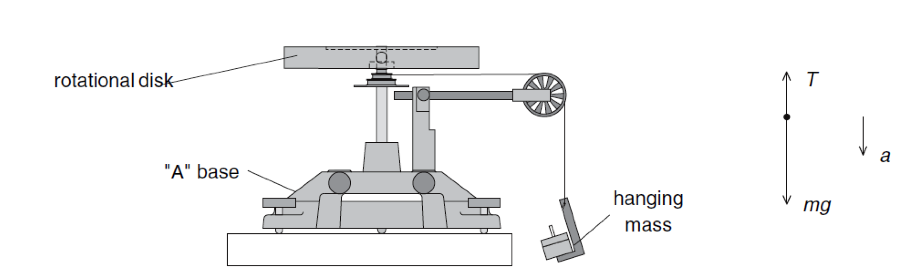
\includegraphics[width=01.0\textwidth]{./Exp6/pic/diskwithmass.png}
	\end{center}
	\caption{A setup used to determine the rotational inertia in this experiment.}
	\label{fig:initsetup}
\end{figure}

\noindent{Solving for the tension in the thread gives}

\begin{equation}
|T| = m(|g|- |a|) = m(|g|-|\alpha| r).
\end{equation}

\noindent{If we assume a frictionless system, the net torque would be}

\begin{gather}
\sum \vec \tau = m\vec gr - m \vec \alpha r^{2} = I \vec \alpha \\
I = \frac{m|g|r}{|\alpha|} - mr^2
\end{gather}

\noindent{Once the angular acceleration of the rotating platform is determined the torque can be obtained for the calculation of the rotational inertia.}\myskip

\section{Procedure}
\label{angexp}

\begin{figure}[!h]
	\begin{center}
	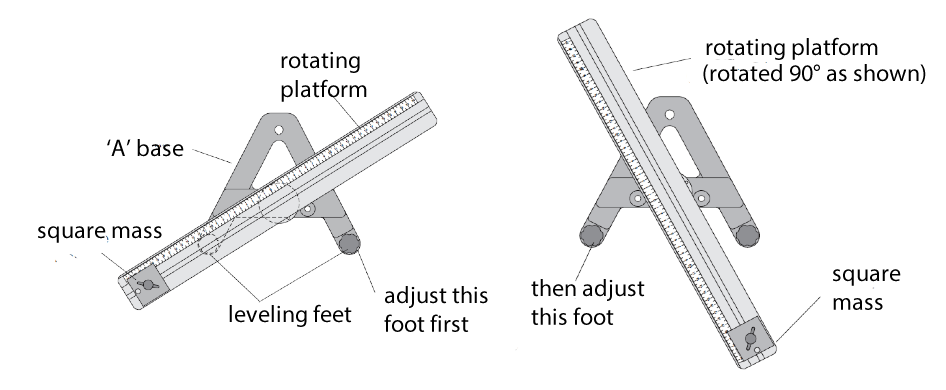
\includegraphics[width=1.0\textwidth]{./Exp6/pic/appbalance2.png}
	\end{center}
\caption{Diagram of the necessary parts to level the apparatus.}
\label{fig:levelapp}
\end{figure}

\subsection{Level the apparatus}
The accuracy needed to correctly measure the moments of inertia requires the apparatus to be extremely level.  To level the base, perform the following steps:

\begin{enumerate}
	\item Adjust the position of the 300 g square mass so that its center is at the 22 cm mark by loosening the screw, sliding the mass along the track, and tightening the screw so the mass will not slide.  Rotate the track until the 300g mass is above the left foot of the ``A'' base, on the same side as the pulley. See the left side of Figure \ref{fig:levelapp}.
	%For some reason, these fig. refs. do not pick up correctly...
	\item Adjust the leveling screw on the side opposite the pulley until the end of the track with the square mass is aligned over the leveling screw on the other leg of the base. See the left side of Figure \ref{fig:levelapp}.
	\item Rotate the track 90 degrees so it is parallel to one side of the ``A" and adjust the other leveling screw until the track will stay in this position. See the right side of Figure \ref{fig:levelapp}.
	\item The track should now be level and should remain at rest in any orientation.
\end{enumerate}

\begin{figure}[b]
	\begin{center}
		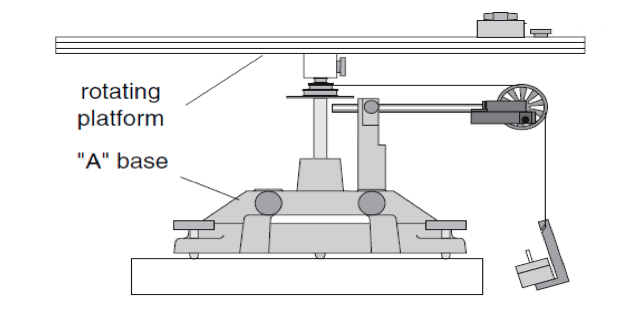
\includegraphics[width=0.6\linewidth]{./Exp6/pic/rotplat.png}
	\end{center}
	\caption{The setup for Section \ref{pointmass}.}
	\label{fig:rotpoint}
\end{figure}

\begin{figure}[h]
	\begin{center}
		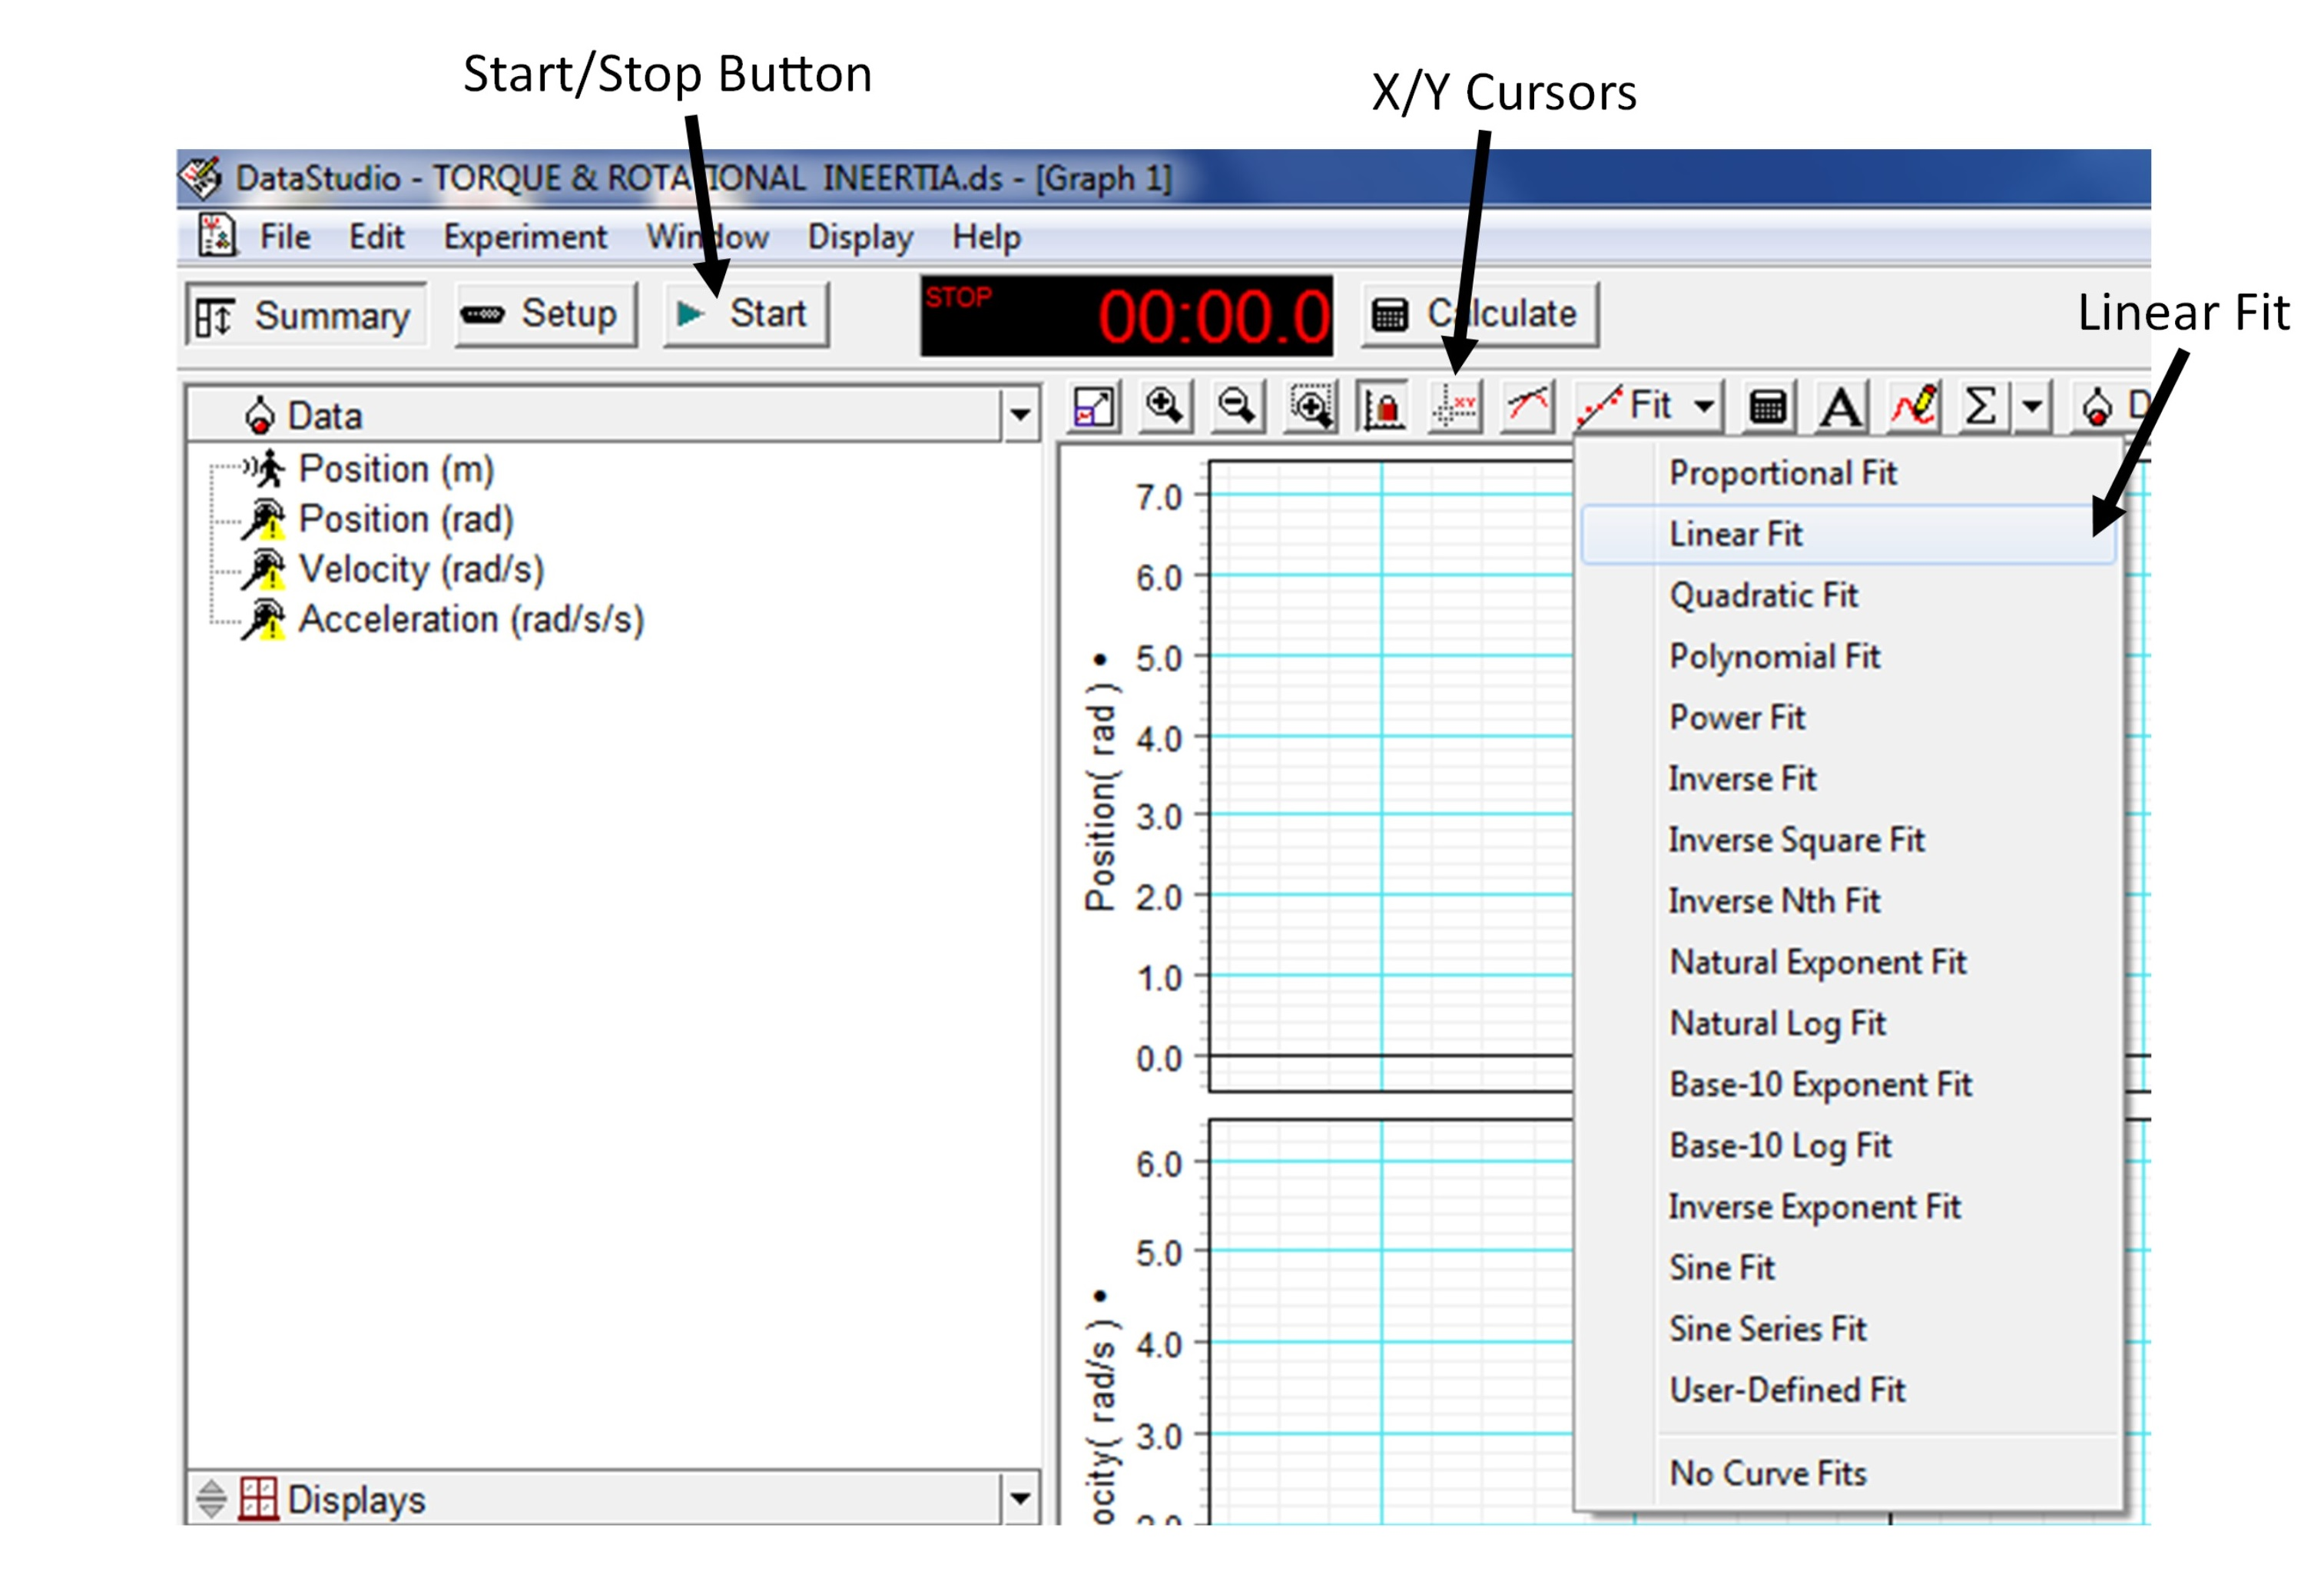
\includegraphics[width=0.9\linewidth]{./Exp6/pic/screenshot1.jpg}
	\end{center}
	\caption{DataStudio Start button.}
	\label{fig:screenshot1}
\end{figure}
\begin{figure}[h]
	\begin{center}
		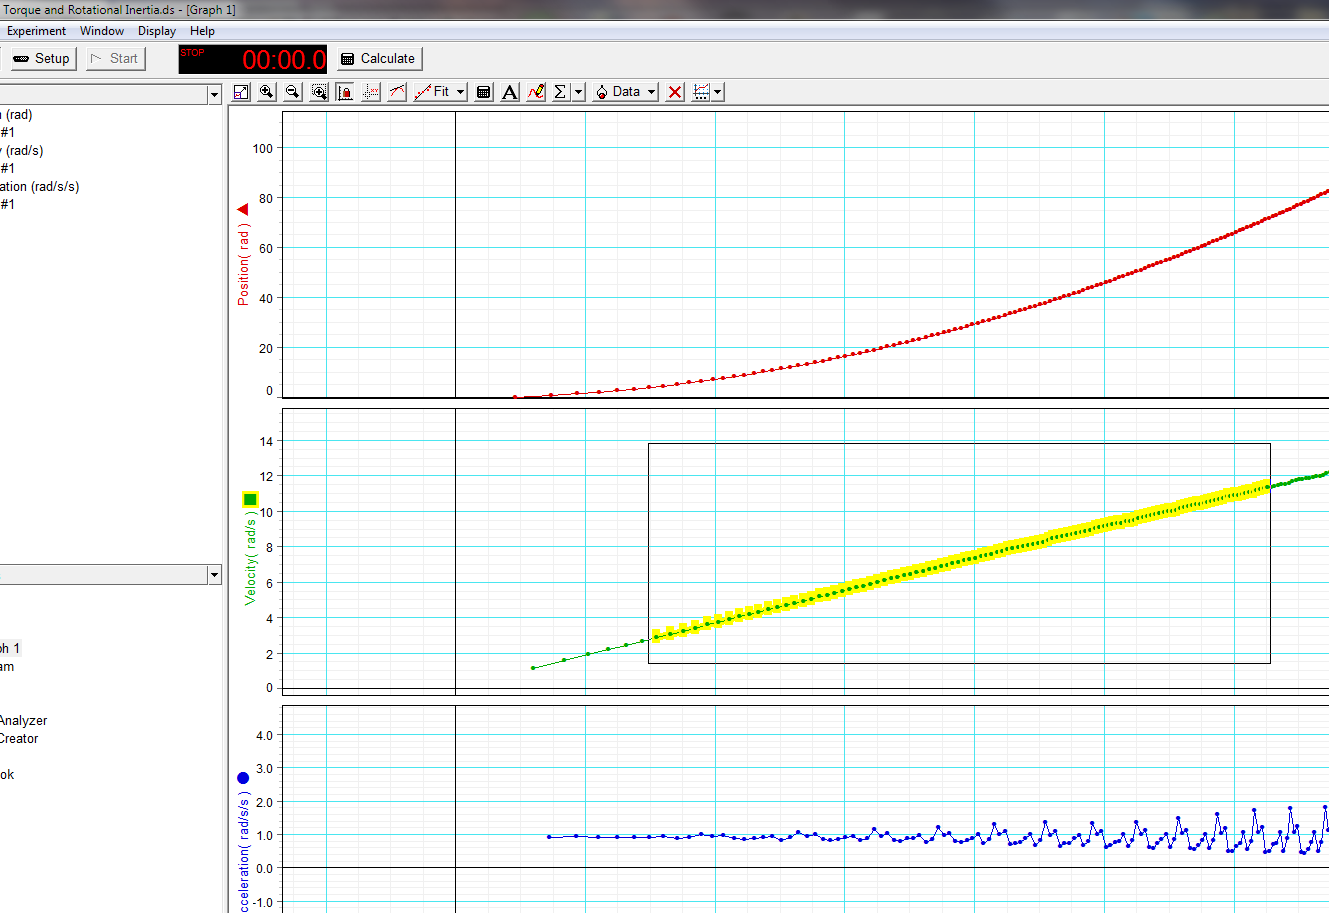
\includegraphics[width=0.9\linewidth]{./Exp6/pic/screenshot2.png}
	\end{center}
	\caption{Selecting data.}
	\label{fig:screenshot2}
\end{figure}
\subsection{Rotational inertia of a point mass}
\label{pointmass}
\begin{enumerate}
	\item With the 300 g square mass still centered on the 22 cm mark, attach a thread to the middle spindle of the step pulley and hang the thread over the 10-spoke pulley.  Allow the string to reach the floor.  Use a caliper to measure the radius of the middle spindle, $r_\text{spindle}$.
	\item Open the ``Torque and Rotational Inertia" DataStudio program.  
	\item Attach a mass to the thread (we suggest $50g$) and wind the middle spindle until the mass is hanging right below the pulley.
	\item Allow the rotating platform to rotate freely and start acquiring data by clicking the "Start" button in DataStudio as shown in Figure \ref{fig:screenshot1}. Stop data acquisition before the mass hits the floor by clicking the same button.
	\item Highlight a linear portion of the angular velocity graph as shown in Figure \ref{fig:screenshot2} and perform a linear fit by clicking the "Fit" drop down menu and selecting "Linear Fit" as shown in Figure \ref{fig:screenshot1}.
	\item Record the slope of the angular velocity graph, which is the average angular acceleration $\alpha _{\rm avg}$, in Table \ref{sectab} in the "300g Mass at 22cm" row and compute the experimental rotational inertia {\it{with error}} found by propagating uncertainties in measured radius $r_\text{spindle}$.
\item Caculate the theoretical rotational inertia of the system $I_\text{theory}$ with error found by propagating uncertainties in radius $R_\text{inertia}$ or length $L$. Record your result in table \ref{firtab}.
	\item Loosen the 300 g mass and slide it along the track until it is centered at the 11 cm mark.  Repeat steps 3 through 7 using the same suspended mass (we suggest $50g$) and fill in Table \ref{firtab} in the "300g Mass at 11cm" row.
	\item Loosen the 300 g mass and remove it from the track.  Repeat steps 3 through 7 using the same suspended mass (we suggest $50g$) and fill in Table \ref{firtab} in the "No Mass on Track" row.
	\item Do your experimentally measured rotational inertia $I_\text{exp}$ agree with your theoretical calculations $I_\text{theory}$ with error? 
\item If your moments of inertia don't agree within error, note the point mass experiments did not use a true point mass. To more accurately calculate the rotational inertia of the point mass experiment try subtracting the "No Mass on the end" rotational inertia from the "300g Mass at 22cm" and the "300g Mass at 11cm" rotational inertias. 
\item Do these new calculate rotational inertias agree with your theoretical calculations $I_\text{theory}$?
\item Discuss which sources of error may contribute to incorrect calculations of the rotational inertia.
\end{enumerate}

\subsection{Rotational inertia of a disk}

\label{diskinert}
\begin{enumerate}
	\item Remove the straight track from the ``A" base by loosening the screw under the track and lifting it from the center shaft.  Put the straight track aside.  Position the rotational disk directly on the center shaft as shown in Figure \ref{fig:rotinertias}.  The side of the disk that has the indentation for the ring should be up.
	\item Attach a hanging mass (we suggest $50g$) to the thread and wind the middle spindle until the mass is hanging right below the pulley.
	\item Allow the rotating platform to rotate freely and start acquiring data.  Stop data acquisition before the mass hits the floor.
	\item Highlight a linear portion of the angular velocity graph and perform a linear fit.
	\item Record the slope of the angular velocity graph (the average angular acceleration $\alpha _{\rm avg}$), in Table \ref{firtab} and compute the experimental rotational inertia {\it{with error}} found by propagating uncertainties in measured radius $r_\text{spindle}$.
\item Caculate the theoretical rotational inertia of the system $I_\text{theory}$ with error found by propagating uncertainties in radius $R_\text{inertia}$ or length $L$. Record your result in table \ref{firtab} in the "Flat Rotational Disk" row.
	\item Remove the disk from the center shaft and rotate it up on its side.  Mount the disk vertically by inserting the shaft in one of the two ``D"-shaped holes on the edge of the disk.  See Figure \ref{fig:rotinertias}.
\item Repeat steps 2 through 6 using the same suspended mass (we suggest $50g$) and fill in Table \ref{firtab} in the "Rotational Disk Side" row.
\item Do your experimentally measured rotational inertia $I_\text{exp}$ agree with your theoretical calculations $I_\text{theory}$ with error? 
\item Discuss which sources of error may contribute to incorrect calculations of the rotational inertia.
\end{enumerate}

\begin{figure}[!h]
	\begin{center}
		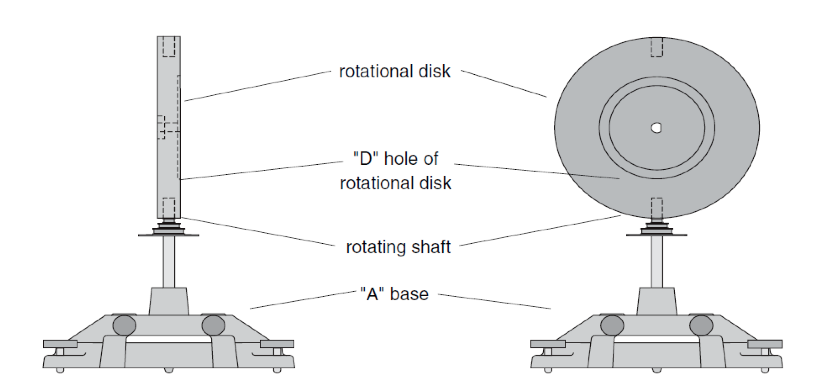
\includegraphics[width=0.8\linewidth]{./Exp6/pic/crazyfig.png}
	\end{center}
	\caption{The setup for Section \ref{diskinert} steps 7 and 8.}
	\label{fig:rotinertias}
\end{figure}

\begin{center}
\begin{table}
\begin{tabular}{| C{4cm} | C{4 cm} | C{4cm} | C{3cm} |}
\hline
\textbf{Shape} & \textbf{Orientation of the Axis} & \textbf{Rotational Inertia} & \textbf{Diagram} \\ \hline
Point Mass & $R$ from point mass & $I = MR^2$ & \\ \hline
Uniform disk with radius $R$ & Through center of disk, perpendicular to the plane of the disk & $I = \frac{1}{2}MR^2$ &\begin{center}
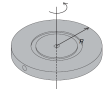
\includegraphics[width=0.6in]{./Exp6/pic/momenti1.png}\end{center}\\ \hline
Uniform disk with radius $R$ & Along diameter of disk & $I = \frac{1}{4}MR^2$ & \begin{center}
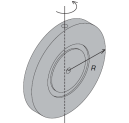
\includegraphics[width=0.6in]{./Exp6/pic/momenti2.png}\end{center}\\ \hline
Uniform ring with inner radius $R_1$ and outer radius $R_2$ & Through center of ring, perpendicular to plane of the ring & $I=\frac{1}{2}M(R_1^2 + R_2^2)$& \begin{center}
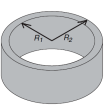
\includegraphics[width=0.6in]{./Exp6/pic/momenti3.png}\end{center}\\ \hline
Uniform rod with length $L$ & Through the center of the rod & $I=\frac{1}{12}ML^2$&\begin{center}
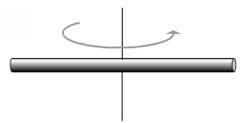
\includegraphics[width=0.6in]{./Exp6/pic/momenti4.png}\end{center}\\ \hline
\end{tabular}
\captionsetup{justification=centering}
\caption{The rotational inertia along with diagrams for various common objects.}
\label{firtab}
\end{table}
\end{center}

\begin{center}
\begin{table}
\begin{tabular}{| C{4.5cm} | C{2.6cm} | C{2.6cm} | C{2.6cm} | C{2.6cm} |}
\hline
Object & $\alpha _\text{avg}$ (rad/s $^{2}$) & $I_\text{exp}$($\text{g} \cdot \text{cm} ^{2}$) & Suspended Mass (g) & $I_\text{theory}$($\text{g} \cdot \text{cm}^2$)\\ \hline
 \textbf{300g Mass at 22cm}& & &&\\ \hline
 \textbf{300g Mass at 11cm}& && &\\ \hline
 \textbf{No Mass on Track}& && &\\ \hline
 \textbf{Flat Rotational Disk}& & &&\\ \hline
 \textbf{Rotational Disk Side} & & &&\\ \hline
\end{tabular}
\captionsetup{justification=centering}
\caption{Data table for various parameters measured in this experiment.}
\label{sectab}
\end{table}
\end{center}